\section{Cardinal Direction Calculus}\label{sec:carddir}

\kasten{
\subsubsection*{Cardinal Direction Calculus overview}
\begin{calcfeatures}
\feature{calculus identifier}{cardir}
\feature{calculus parameters}{none}
\feature{arity}{binary}
\feature{entity type}{2D points}
\feature{description}{describes the orientation of two point regarding and absolute orientation}
\feature{base relations}{N, NE, E, SE, S, SW, W, NW, EQ}
\lastfeature{references}{\citet{frank-ACSM:91}, \citet{ligozat98_carddir}}
\end{calcfeatures}
}


\citet{frank-ACSM:91} introduced the cardinal direction calculus.%
\footnote{\citeauthor{frank-ACSM:91} introduced two different variants, called projection-based and cone-based. This calculus definition implements the projection-based variant.}
The euclidian plane $\mathcal{P}$ is partitioned into regions
with respect to a reference point $R$ and a global
\emph{west-east/south-north} reference frame.
Any point $P\in\mathcal{P}$ belongs to
one of the nine basic relations:
\textbf{N}orth, \textbf{N}orth\textbf{E}ast,
\textbf{E}ast, \textbf{S}outh\textbf{E}ast,
\textbf{S}outh, \textbf{S}outh\textbf{W}est,
\textbf{W}est, \textbf{N}orth\textbf{W}est,
or \textbf{Eq}ual.
The model is depicted in Figure \ref{fig:CardDir}.

\begin{figure}[htp]
	\centering
	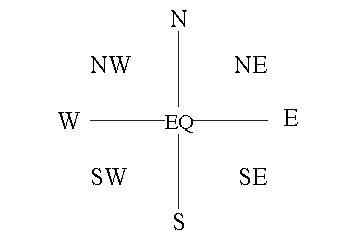
\includegraphics[width=0.5\textwidth]{CardDir_Projection}
	\caption{Base relations of the cardinal direction calculus.}
	\label{fig:CardDir}
\end{figure}

